\chapter{Scaling Functions}
\label{annex:functions}
As the metrics are aggregated to compute the QoI, their values need to be on the same scale. In order to do this, we use scaling functions rescaling metrics into a range of $[-1,1]$, as the QoI bounds. As all the metrics does not have the same properties, they have to be scaled by using different functions. The two properties to check to choose which function to apply to which metric are the following ones:
\begin{itemize}
	\item does the metric already have a bounded value ?
	\item what value of the metric should make the QoI decrease, increase or remain the same ?
\end{itemize}
Therefore, we designed three functions to be used with metrics having bounded values and three functions for metrics that do not have upper bounds. Then, among these two sets of functions, it is possible to choose the one to use according to the positive, neutral or negative impact a value should have on the QoI.

\section{Scaling of bounded metrics: Min-Max Normalization} \label{subsubsec:norma} We defined three min-max normalization functions, illustrated in Fig.~\ref{fig:norma}. They were designed to be used for metrics whose values belong to a bounded set, \ie metrics for which the minimum and maximum values are known. The first function is to apply in cases for which a measure approaching the bound value $b_1$ has a negative impact on the quality evaluation whereas a measure approaching $b_2$ has a positive one. It allows to scale a measure $x$ between -1 and 1:
\begin{equation}\label{eq:norma1}
n_1(x) = 2 * \dfrac{x-b_1}{b_2-b_1} -1
\end{equation}
The second function is intended to be applied in cases for which a measure approaching the bound value $b_1$ has a neutral impact on the quality evaluation whereas a measure approaching $b_2$ has a positive one. It allows to scale a measure $x$ between 0 and 1:
\begin{equation}\label{eq:norma2}
n_2(x) = \dfrac{x-b_1}{b_2-b_1}
\end{equation}
Finally, the last function is to apply in cases for which a measure approaching the bound value $b_1$ has an negative impact on the quality evaluation whereas a measure approaching $b_2$ has a neutral one. It allows to scale a measure $x$ between -1 and 0:
\begin{equation}\label{eq:norma3}
n_3(x) = \dfrac{x-b_2}{b_2-b_1}
\end{equation}
\begin{figure}[!htp]
	\centering
	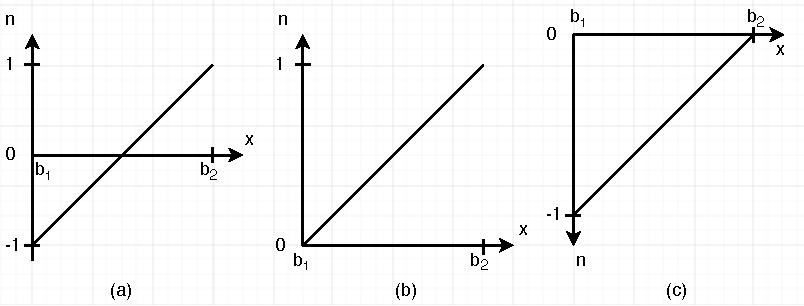
\includegraphics[width=\linewidth]{figures/annexe1/norma.pdf}
	\caption{(a), (b) and (c) respectively represent the min-max normalization functions \eqref{eq:norma1}, \eqref{eq:norma2} and \eqref{eq:norma3}}
	\label{fig:norma}
\end{figure}

\section{Scaling of unbounded metrics: Sigmoid Normalization}\label{subsubsec:loga}
We defined three sigmoid-like functions to scale and squash values of metrics without an upper bound. As for the min-max normalization, there is one function to scale the metrics values between -1 and 1, another one to scale between 0 and 1 and the last one to scale between -1 and 0. 

The first function allows to scale between -1 and 1 the values of a metric, for a metric whose values are between 0 and $+\infty$ (e.g. a duration whose final value is unknown during the execution). The function is defined as:
\begin{equation}\label{eq:sig1}
s_1(x) = 1 - 2 \exp{\left(-\ln{(2)}\left(\dfrac{x}{th}\right)^k\right)}, x > 0
\end{equation}
with $s_1(x) \in [-1,1]$, $th$ the value of the sigmoid's midpoint (\ie $s_1(th)=0$) and, $k$ setting the shape of the function curve. $k$ and $th$ values are set off-line by the designer and they allow to define the shape of the metric scaling.

The second function is designed for metric which cannot have a negative impact on the QoI as it scales the value between 0 and 1 (and with $x \in [0,+\infty]$ as well):
\begin{equation}\label{eq:sig2}
s_2(x) = 1 - \exp{\left(-\ln{(2)}\left(\dfrac{x}{th}\right)^k\right)}, x > 0
\end{equation}
with $s_2(x) \in [0,1]$, $th$ the value of the sigmoid's midpoint (\ie $s_2(th)=0.5$) and, $k$ setting the shape of the function curve.

The third function is designed for metric which cannot have a positive impact on the QoI as it scales the value between -1 and 0 (and with $x \in [0,+\infty]$ as well):
\begin{equation}\label{eq:sig3}
s_3(x) = - 1 + \exp{\left(-\ln{(2)}\left(\dfrac{x}{th}\right)^k\right)}, x > 0
\end{equation}
with $s_3(x) \in [-1,0]$, $th$ the value of the sigmoid's midpoint (\ie $s_3(th)=-0.5$) and, $k$ setting the shape of the function curve.

The functions $s_1(x)$ and $s_2(x)$ are illustrated in Fig.~\ref{fig:chart} with four examples.
\begin{figure}[!htp]
	% Maximum length
	\subfloat[Plot of $s_1(x)$ with $th=3$ and $k=2$]{\label{fig:chart6}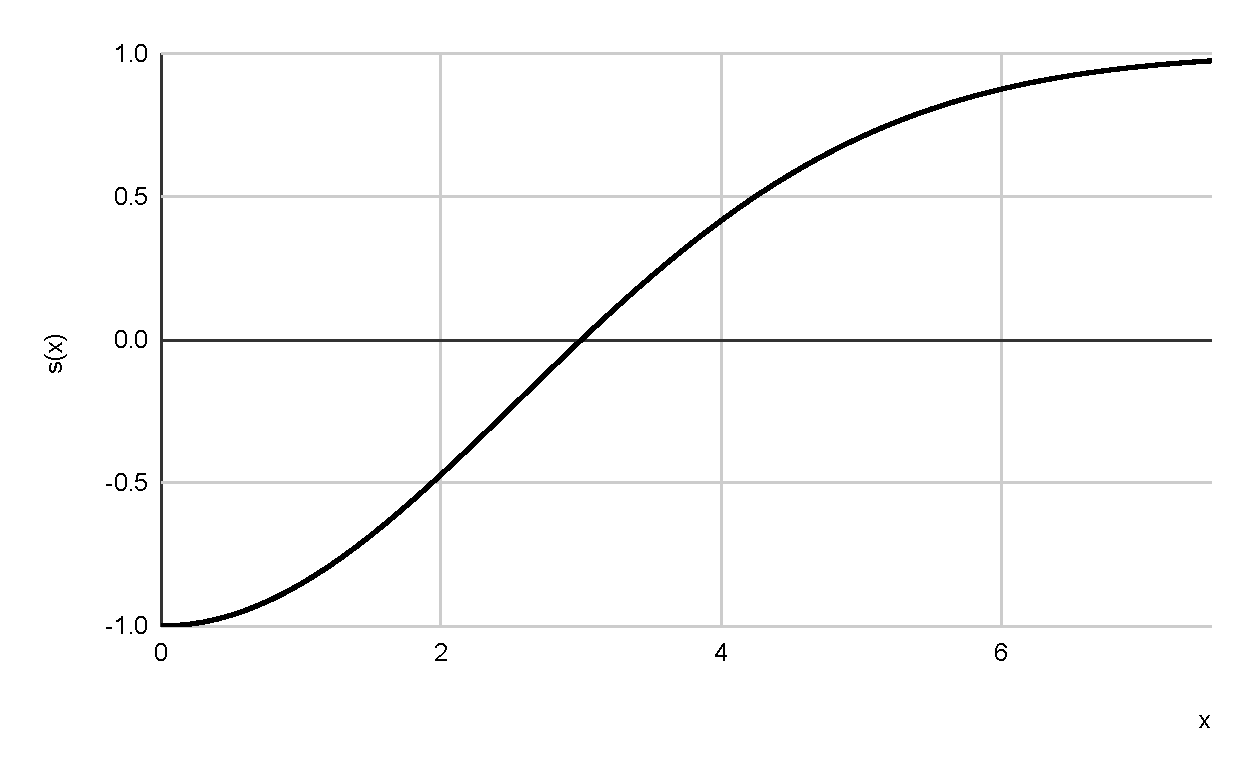
\includegraphics[scale=0.4]{figures/annexe1/chartsx6.pdf}}\hfill
	\subfloat[Plot of $s_2(x)$ with $th=3$ and $k=1$]{\label{fig:chart3}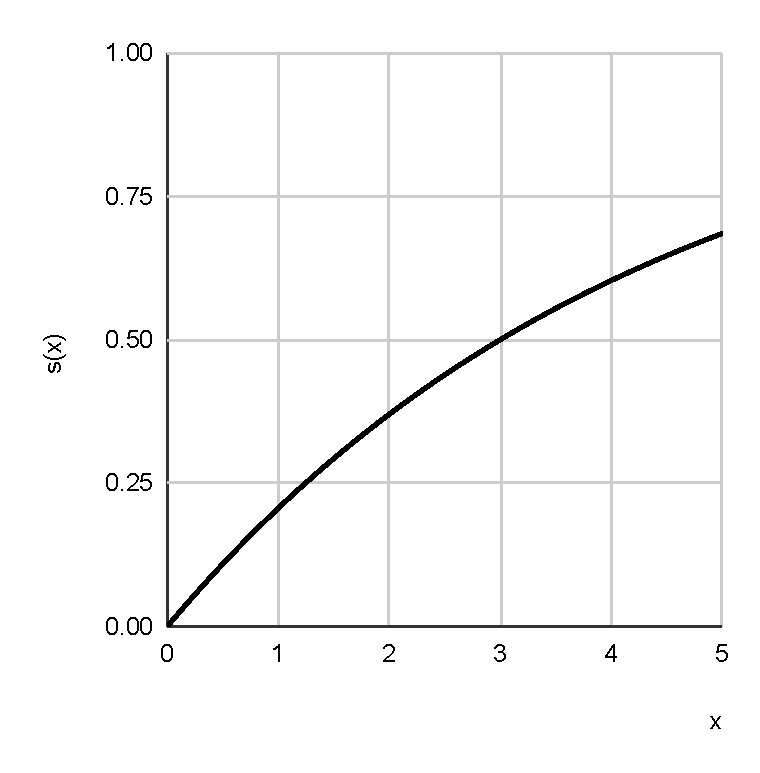
\includegraphics[scale=0.4]{figures/annexe1/chartsx2.pdf}}\hfill
	\subfloat[Plot of $s_2(x)$ with $th=3$ and $k=2$]{\label{fig:chart1}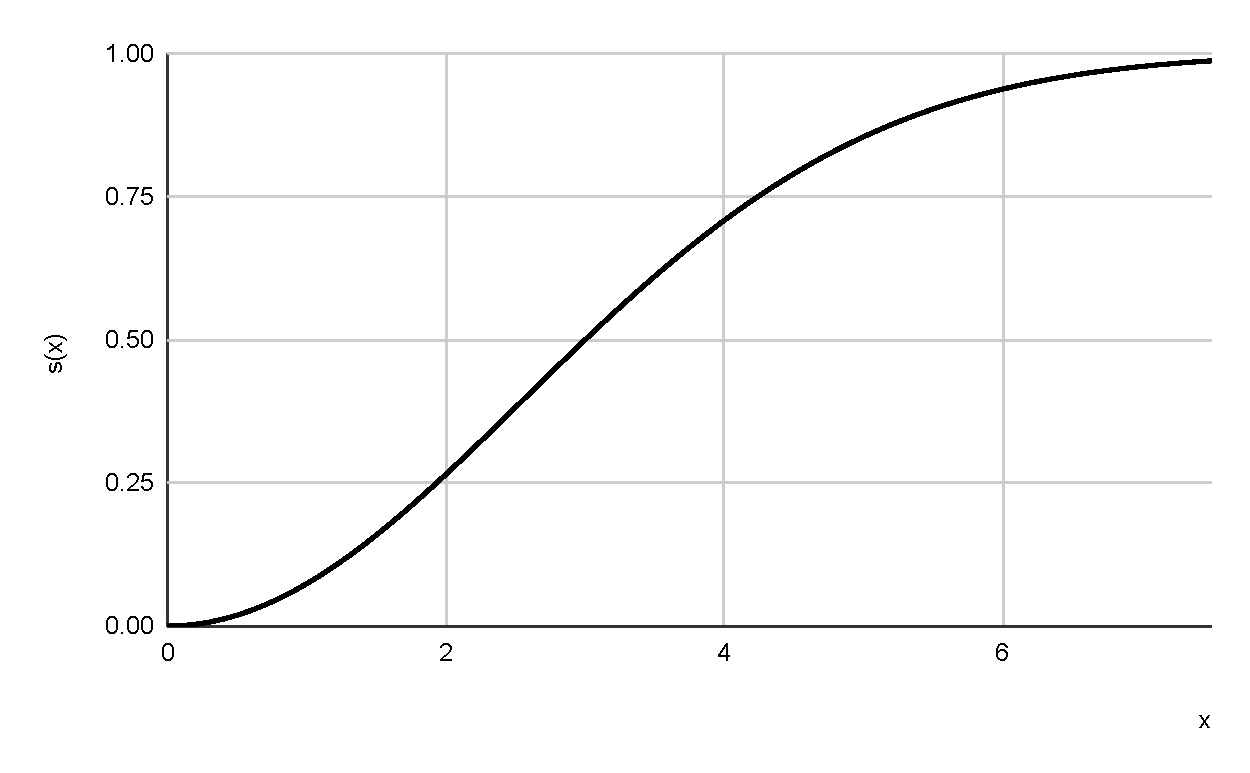
\includegraphics[scale=0.4]{figures/annexe1/chartsx3.pdf}}\hfill
	\subfloat[Plot of $s_2(x)$ with $th=0.5$ and $k=2$]{\label{fig:chart2}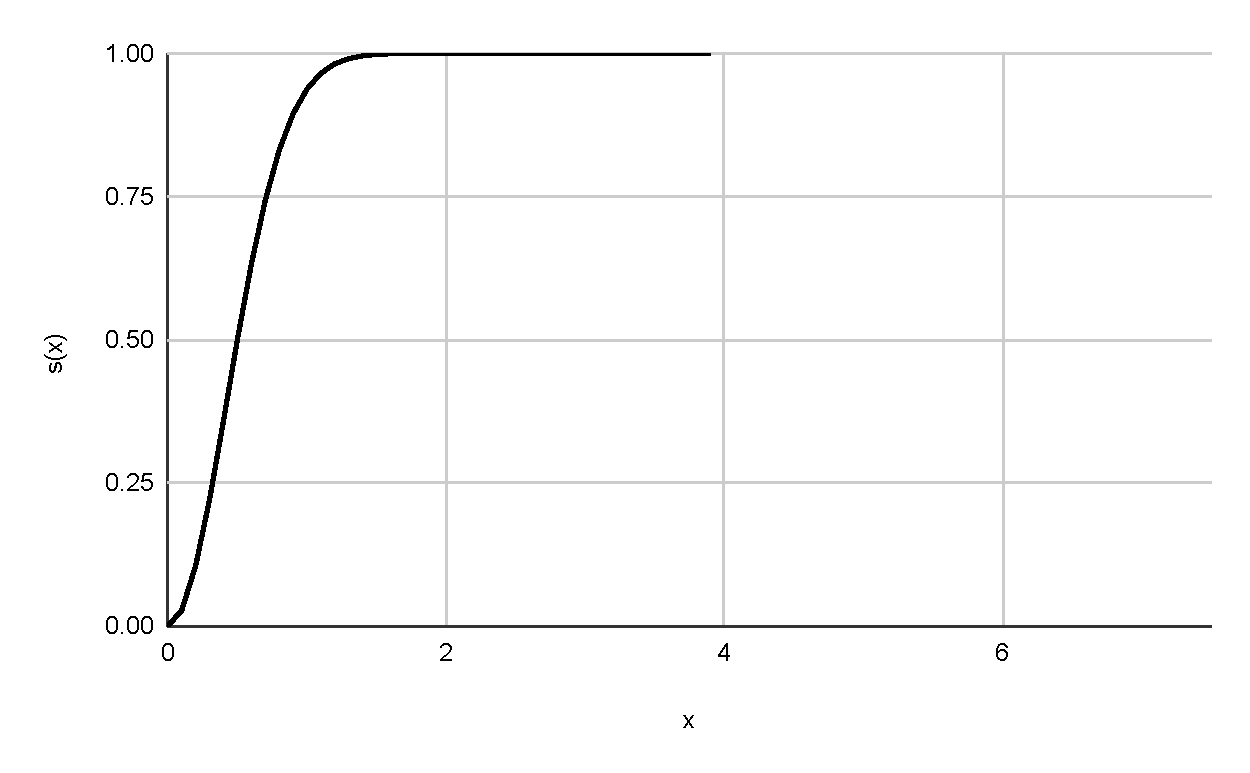
\includegraphics[scale=0.4,trim={0 0 7cm 0},clip]{figures/annexe1/chartsx4.pdf}}\hfill
	
	\caption{Plots of the sigmoid-like functions $s_1(x)$ and $s_2(x)$ with different parameters values}
	\label{fig:chart}
\end{figure}


